\section{Capítulo 8, Tsamparlis (2019)}

Dado que la teoría de la relatividad especial es claramente inconsistente con nuestra experiencia diaria, se pueden "crear" experimentos hipotéticos (mentales) para contrastar la "nueva" teoría con la newtoniana. Todo esto incluyendo, la contracción de la longitud y la dilatación del tiempo. A estos experimentos se les conocen como paradojas. Las paradojas son construidas mediante situaciones comunes (newtonianas) llevadas al "terreno" relativista.

\subsection{Paradoja de la Lámpara}
Esta paradoja toma el circuito (\ref{lamp}) el conjunto $CEDZ$, que se encuentra en el circuito $\Sigma$, se mueve con velocidad $\beta c$ hacia la derecha, la corriente únicamente corre por los segmentos $CE$ y $DZ$; además, $CD = AB$. Tomando $\Sigma$ el observador propio en el complejo $CEDZ$. De acuerdo a $\Sigma$ la distancia $CD < AB$, de modo que la lámpara estará apagada cierto tiempo; mientras que para $\Sigma '$ $AB < CD$, de modo que la lámpara siempre está encendida. La idea de este escenario es probar que estó físicamente es cierto y no constituye una paradjoa como tal. 

\begin{figure}[H]
	\centering
	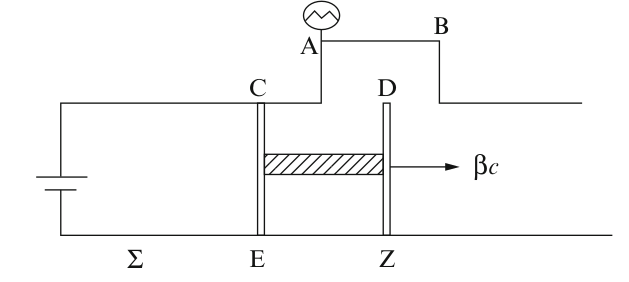
\includegraphics[scale=0.5]{img/lamp.png}
	\caption{Circuito de la paradoja de la lámpara.}
	\label{lamp}
\end{figure}

La idea de la demostración radíca en la velocidad de propagación del campo electromagnetico en el conductor. En base a esta idea se plantean las respectivas ecuaciones de contracción de la longitud para cada uno de los sistemas. Ya teniendo esto, se concluye que si la lámpara se apaga para $\Sigma$ también lo hace para $\Sigma '$ en periodos de tiempo relacionados con la fórmula siguiente: $T_{off} ' = \gamma T_{off}$.

\subsection{Paradoja de la Sombra}
Tenemos una fuente de luz monocromática a una altura $h_s$ y un muro de grosor despresiable con altura $h_w < h_s$. La sombra generada por la fuente y el muro se achica conforme la fuente se acerca al muro, haciendola desaparecer cuando se encuentra directamente sobre él. La idea del planteamiento de la paradoja es tomar una velocidad $u$ tal que $\frac{u}{c} > 1 - \frac{h_w}{h_s}$, de modo que la sombra desaparece incluso antes de que la fuente llegue a estar sobre el muro.

\begin{figure}[H]
	\centering
	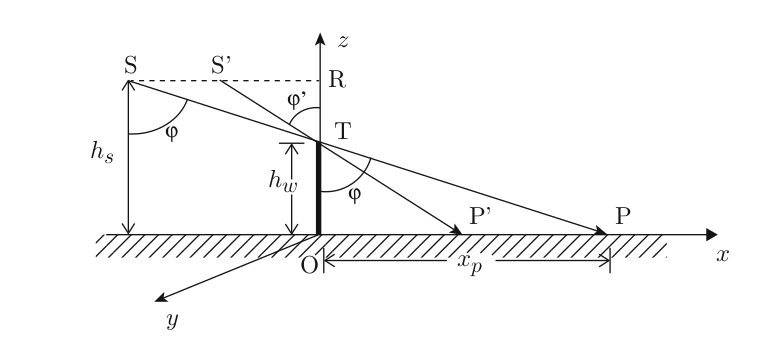
\includegraphics[scale=0.5]{img/light.png}
	\caption{Paradoja de la sombra.}
	\label{shadow}
\end{figure}


\subsection{Perímetro del Triángulo Equilátero}
Se tiene un triángulo moviendose a velocidad relativista paralelo a uno de sus lados o paralelo a una de sus alturas. Dada la contracción lorentz el perímetro del triángulo se reducirá en cierto factor dependiente de la velocidad $u$. Lo interesante no es el perímetro en sí, sino ver el comportamiento del mismo en los límites $u \ll c$ y $u\approx c$.

\subsection{Paradoja de los Gemelos}
Esta es la paradoja más utilizada en divulgación científica. Fue propuesta por Paul Langevin, en esta paradoja se plantea a un par de gemelos en un sistema $\Sigma$, y uno de ellos se empieza a mover con velocidad constante en cierto periodo de tiempo, igual, respecto a $\Sigma$, luego cambia instantaneamente de dirección regresando al punto de partida en $\Sigma$. El resultado es que el gemelo que viajo, vuelve más joven que el que permaneció en reposo en $\Sigma$.














%%%%%%%%%%%%%%%%%%%%%%%%%%%%%%%%%%%%%%%%%%%%%%%%%%%%%%%%%%%%%%%